\begin{figure}[H]
	\begin{minipage}[t]{0.45\linewidth}
	\centering
	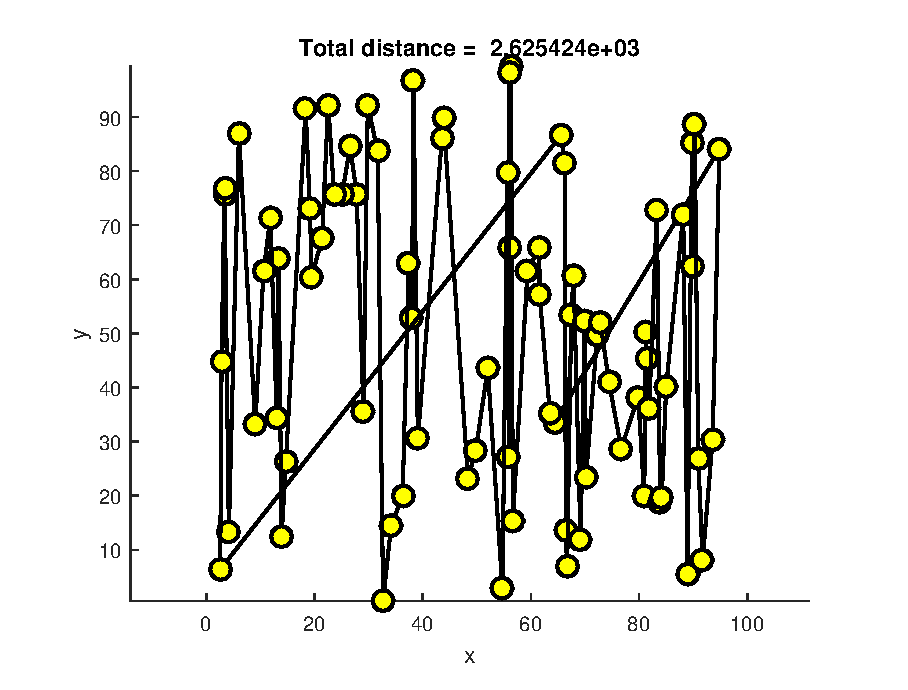
\includegraphics[width=\textwidth]{\Pathofcities/path.eps}
	\caption{Path journey}\label{fig:Pathofcities:path}
	
	\end{minipage}\hfill
	\begin{minipage}[t]{0.45\linewidth}
	\centering
	\includegraphics[width=\textwidth]{\Pathofcities/AS_1_5AS_ExecTimeAndMeanSTDWith_execVariation.eps}
	\caption{Variation of the execution time VS the \# of ants (20$\stackrel{step=20}{\rightarrow}$100) in each execution (1$\stackrel{step=1}{\rightarrow}$ 5)}
	\label{fig:Pathofcities:AS_1_5AS_ExecTimeAndMeanSTDWith_execVariation}
	\end{minipage}
	\flushleft
	\begin{minipage}[t]{0.45\linewidth}
	\centering
	\includegraphics[width=1.5\textwidth,height=.9\textwidth]{\Pathofcities/AS_BestCost_Varying_Iteration_and_nbAnts.eps}
	\caption{Best cost VS Ants number variation with $\alpha$=1, $ \beta $ = 5}
	\label{fig:Pathofcities:AS_BestCost_Varying_Iteration_and_nbAnts}
	\end{minipage}
%%	\vspace{length}
\end{figure}\flushright
	\begin{minipage}[t]{0.9\linewidth}
	\vspace{-9mm}
	\begin{table}[H]
	\label{tab:Pathofcities:expdeux}
	\begin{tabular}{lllll}
	\cline{1-2}
	\multicolumn{1}{|l|}{Best Costs results for experience 2 on cities.dat }                                                           &  \multicolumn{1}{l|}{Elapsed Time, Mean, STD}                                             &  &  &  \\ \cline{1-2}
	\multicolumn{1}{|l|}{\begin{tiny}\begin{tabular}{|l|c|c|c|c|c|c|c|c|c|c|}
\hline
&\textbf{It :1}&\textbf{It :2}&\textbf{It :3}&\textbf{It :4}&\textbf{It :5}&\textbf{It :6}&\textbf{It :7}&\textbf{It :8}&\textbf{It :9}&\textbf{It :10}\\\hline
\textbf{exec :1}&28.07&28.07&28.07&28.07&28.07&28.07&28.07&27.52&27.52&27.52\\\hline
\textbf{exec :2}&28.86&28.86&28.86&28.86&28.86&28.86&27.52&27.52&27.52&27.52\\\hline
\textbf{exec :3}&29.16&29.13&28.05&28.05&28.05&28.05&28.05&28.05&27.72&27.52\\\hline
\textbf{exec :4}&29.05&27.52&27.52&27.52&27.52&27.52&27.52&27.52&27.52&27.52\\\hline
\textbf{exec :5}&29.47&27.52&27.52&27.52&27.52&27.52&27.52&27.52&27.52&27.52\\\hline
\textbf{exec :6}&28.66&28.09&27.52&27.52&27.52&27.52&27.52&27.52&27.52&27.52\\\hline
\textbf{exec :7}&28.05&27.72&27.52&27.52&27.52&27.52&27.52&27.52&27.52&27.52\\\hline
\textbf{exec :8}&27.72&27.52&27.52&27.52&27.52&27.52&27.52&27.52&27.52&27.52\\\hline
\textbf{exec :9}&27.52&27.52&27.52&27.52&27.52&27.52&27.52&27.52&27.52&27.52\\\hline
\textbf{exec :10}&27.52&27.52&27.52&27.52&27.52&27.52&27.52&27.52&27.52&27.52\\\hline
\end{tabular}
\end{tiny}} & \multicolumn{1}{l|}{\begin{tiny}\begin{tabular}{|l|c|}
\hline
&\textbf{Elapsed time}\\\hline
\textbf{exec :1}&0.29\\\hline
\textbf{exec :2}&0.54\\\hline
\textbf{exec :3}&0.78\\\hline
\textbf{exec :4}&1.02\\\hline
\textbf{exec :5}&1.27\\\hline
\textbf{exec :6}&2.48\\\hline
\textbf{exec :7}&3.73\\\hline
\textbf{exec :8}&4.96\\\hline
\textbf{exec :9}&6.16\\\hline
\textbf{exec :10}&12.40\\\hline
\textbf{ Mean}&3.36\\\hline
\textbf{ STD}&3.75\\\hline
\end{tabular}
\end{tiny} } &  &  &  \\ \cline{1-2}
	&     &  &  &  \\
	&     &  &  & 
	\end{tabular}
	\caption{Results of experience 2 on cities.dat}
	\end{table}
	\end{minipage}

%%\end{figure}